\section{Introduction}

\IEEEPARstart{B}{iomedical} artificial intelligence works in a domain where knowledge is large, heterogeneous, contested, time-dependent, and consequential. A single clinical or scientific question can connect symptoms, diseases, drugs, genes, pathways, trials, guidelines, laboratory observations, and patient context. The relevant facts sit across terminologies, curated databases, publications, electronic health records (EHRs), and local protocols. They also differ in evidential strength, and they go out of date. These properties make biomedicine a natural but demanding setting for joining knowledge graphs (KGs) with large language models (LLMs).

A biomedical KG represents entities and typed relations in an explicit graph. Depending on its purpose it may encode ontology-backed concepts, literature-derived assertions, experimentally observed associations, patient events, or some mix of these. Resources such as Hetionet~\cite{himmelstein2017hetionet}, SPOKE~\cite{morris2023spoke}, the Clinical Knowledge Graph~\cite{santos2022ckg}, PrimeKG~\cite{chandak2023primekg}, iKraph~\cite{zhang2025ikraph}, and PubMed Knowledge Graph 2.0~\cite{xu2025pubmedkg} trace the field's move from individual relation datasets toward large, multimodal, provenance-bearing knowledge infrastructures. LLMs provide the complementary half: a general interface for interpreting questions, mapping language to concepts and tools, synthesizing evidence, and producing explanations. Their weaknesses matter just as much. Parametric knowledge can be stale or unverifiable, generated claims may be unsupported, confidence expressed in prose is poorly calibrated, and reasoning that looks plausible can hide a retrieval, logic, or data error.

The pairing is attractive because the parts look complementary. A graph can supply explicit semantics, neighborhood structure, paths, constraints, and source attribution. An LLM can translate natural language into graph operations, select and verbalize subgraphs, propose candidate relations, and lower the expertise needed to query a complex resource. That complementarity has produced several method families: graph retrieval-augmented generation (GraphRAG), including deterministic variants built for mechanistic traceability~\cite{pramanik2026mechanistic}, natural-language-to-SPARQL or Cypher interfaces, graph-conditioned prediction via multimodal transformers~\cite{das2025drugmap}, frequency-based graph traversal for drug-effect classification~\cite{chanda2026drugeffect}, graph-aware fine-tuning, KG-constrained decoding, LLM-assisted entity and relation extraction, ontology alignment, graph completion, graph repair, and tool-using agents that alternate between retrieval, reasoning, and graph revision.

The intuitive case has too often stood in for an empirical one. A retrieved path is not necessarily relevant. A relevant path is not necessarily used by the model. A fluent rationale is not necessarily faithful to the path or the answer. A citation is not necessarily evidence for the sentence it follows. The 2026 frontier makes these distinctions hard to ignore. A multi-model biomedical RAG study found the improvements small and inconsistent across datasets and retrieval settings, and it named evidence use, not retrieval alone, as the central bottleneck~\cite{nourbakhsh2026retrieval}. VERICITE found low sentence-level support among retrieved citation-claim pairs and showed that adding retrieval depth could make citation faithfulness worse~\cite{ma2026vericite}. The temporal evaluation in ChronoMedKG reported a sharp fall from static to time-sensitive questions, with graph retrieval recovering only part of the loss~\cite{ahmed2026chronomedkg}. MHGraphBench reported that a graph snippet can help one model and distract another, which makes graph textualization and context management part of the method rather than a neutral implementation detail~\cite{liu2026mhgraphbench}. None of this argues against graphs. It shows that ``KG-augmented'' is an intervention whose mechanism and boundary conditions have to be measured.

The survey literature is itself getting crowded. Xu et al.~\cite{xu2025biomedklm} organize biomedical KG--LLM work around LLM-aided KG construction, KG-guided LLM enhancement, and applications. Murali et al.~\cite{murali2026integrating} separate KG-enhanced LLMs, LLM-augmented KGs, and synergistic systems. A systematic review and meta-analysis has already assessed retrieval-augmented generation across biomedicine~\cite{liu2025biomedrag}, and preprint reviews cover biomedical RAG~\cite{he2025biomedrag} and biomedical KGs more broadly~\cite{lu2025biomedkg}. Directionality is still useful. It is no longer a sufficient novelty claim or a sufficient analytical frame.

This survey therefore treats biomedical KG--LLM integration as an end-to-end engineered and governed lifecycle. Its contributions are fivefold.

\begin{enumerate}
\item \emph{A multidimensional taxonomy.} We classify systems by knowledge-flow direction, lifecycle stage, coupling depth, knowledge object, and evidence maturity, rather than assuming that all ``graph grounding'' works the same way.
\item \emph{An evidence-critical method synthesis.} We analyze graph-to-LLM, LLM-to-graph, and closed-loop systems in terms of mechanisms, dependencies, tradeoffs, failure propagation, and suitable baselines.
\item \emph{A resource and benchmark map.} We compare biomedical KGs, ontologies, clinical data resources, tasks, and emerging graph-reasoning benchmarks, with explicit attention to licensing, provenance, versioning, temporal support, and target leakage.
\item \emph{A layered evaluation framework.} We separate graph, retrieval, reasoning, generation, system, human, clinical, and deployment measures, and we specify the ablations and stress tests needed to establish that the graph itself causes a benefit.
\item \emph{A translation and governance framework.} We introduce an evidence-maturity ladder and a hazard-control-verification model for provenance, privacy, security, interoperability, human oversight, change management, and circular self-validation.
\end{enumerate}

The intended audience spans machine learning, knowledge representation, biomedical informatics, and clinical AI. The conclusion is deliberately bounded. KGs can improve biomedical LLM systems when their coverage, update policy, retrieval mechanism, representation, and verification process fit the task. They do not confer factuality, explainability, or safety by their presence alone. Fig.~\ref{fig:abstract} summarizes the argument, and Fig.~\ref{fig:roadmap} maps the sections that develop it.

% Graphical abstract: what the paper does.
\begin{figure*}[!t]
\centering
\resizebox{\textwidth}{!}{%
\begin{tikzpicture}[
  font=\small,
  hdr/.style={font=\small\bfseries, align=center},
  ax/.style={draw=black!60, rounded corners=2pt, fill=blue!7,
             text width=34mm, align=center, minimum height=8mm, inner sep=3pt},
  lay/.style={draw=black!60, rounded corners=2pt, fill=teal!9,
              text width=34mm, align=center, minimum height=8mm, inner sep=3pt},
  fail/.style={draw=orange!70!black, rounded corners=2pt, fill=orange!12,
               text width=34mm, align=center, minimum height=8mm, inner sep=3pt},
  big/.style={-{Stealth[length=4mm]}, line width=1.6pt, draw=black!40}
]

% ---- column 1: five classification axes
\node[hdr] (h1) at (0,1.35) {How systems are classified};
\node[ax] (a1) at (0,0.35)   {Direction of knowledge flow};
\node[ax] (a2) at (0,-0.85)  {Lifecycle stage};
\node[ax] (a3) at (0,-2.05)  {Coupling depth};
\node[ax] (a4) at (0,-3.25)  {Knowledge object};
\node[ax] (a5) at (0,-4.45)  {Evidence maturity};

% ---- column 2: seven evaluation layers
\node[hdr] (h2) at (6.2,1.35) {Where benefit is measured};
\node[lay] (l1) at (6.2,0.55)   {Graph and schema};
\node[lay] (l2) at (6.2,-0.45)  {Linking and query};
\node[lay] (l3) at (6.2,-1.45)  {Retrieval};
\node[lay] (l4) at (6.2,-2.45)  {Evidence use};
\node[lay] (l5) at (6.2,-3.45)  {Generation};
\node[lay] (l6) at (6.2,-4.45)  {Systems cost};
\node[lay] (l7) at (6.2,-5.45)  {Human utility};

% ---- column 3: failure modes
\node[hdr] (h3) at (12.4,1.35) {Why it fails in practice};
\node[fail] (f1) at (12.4,0.35)  {Coverage gaps, stale edges};
\node[fail] (f2) at (12.4,-0.85) {Entity-linking error};
\node[fail] (f3) at (12.4,-2.05) {Context dilution};
\node[fail] (f4) at (12.4,-3.25) {Unsupported citation};
\node[fail] (f5) at (12.4,-4.45) {Circular self-validation};

% ---- flow arrows between columns
\draw[big] (2.05,-2.05) -- (4.15,-2.05);
\draw[big] (8.25,-2.05) -- (10.35,-2.05);

% ---- conclusion strip
\node[draw=black!55, fill=blue!5, rounded corners=2pt, text width=168mm,
      align=center, inner sep=5pt, font=\small] at (6.2,-7.1)
  {\textbf{Bounded finding.} A graph helps when it holds knowledge the model lacks, entity linking
   succeeds, retrieval returns a compact and relevant subgraph, and the comparison is a matched
   text-retrieval baseline. Otherwise it adds cost, and sometimes error.};
\end{tikzpicture}%
}
\caption{The structure of this survey's argument. \textbf{Left:} systems are classified along five axes rather than by direction of knowledge flow alone, because pasting triples into a prompt and training a graph-aware encoder are different interventions that the usual taxonomy treats alike. Coupling depth runs from C0, where graph and model share an application but exchange nothing structured, to C5, where the graph constrains decoding and may receive controlled write-back; evidence maturity runs from E0, a prototype with no systematic evaluation, to E6, governed routine use. \textbf{Centre:} benefit is measured at seven separable layers, L1 through L7 in the order shown, so that a failure can be attributed to the graph, the linker, the retriever, or the generator rather than to the system as a whole. \textbf{Right:} the failure modes that recur across the reviewed systems. Circular self-validation arises only in closed-loop designs that write model output back into the graph, and it has no analogue in unidirectional systems.}
\label{fig:abstract}
\end{figure*}

% Hierarchical roadmap of the survey's contents.
\begin{figure*}[!t]
\centering
\resizebox{\textwidth}{!}{%
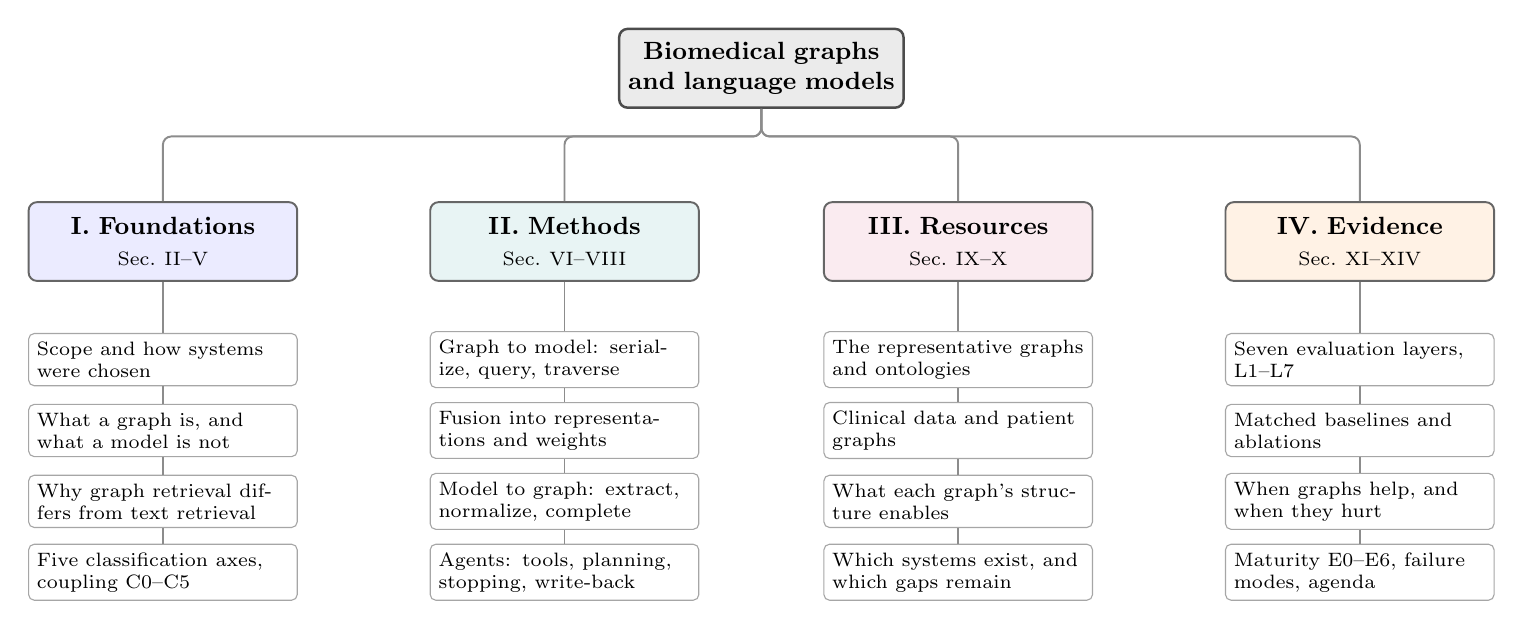
\begin{tikzpicture}[
  font=\small,
  root/.style={draw=black!70, rounded corners=3pt, fill=black!8, text width=34mm,
               align=center, minimum height=10mm, inner sep=3pt, line width=0.9pt},
  part/.style={draw=black!60, rounded corners=3pt, text width=32mm,
               align=center, minimum height=10mm, inner sep=3pt, line width=0.7pt},
  pA/.style={part, fill=blue!8},
  pB/.style={part, fill=teal!9},
  pC/.style={part, fill=purple!8},
  pD/.style={part, fill=orange!10},
  leaf/.style={draw=black!35, rounded corners=2pt, fill=white, text width=32mm,
               align=left, inner sep=3pt, font=\scriptsize},
  e/.style={draw=black!45, line width=0.7pt, rounded corners=3pt}
]

% root
\node[root] (root) at (7.6,1.6) {\textbf{Biomedical graphs and language models}};

% four parts
\node[pA] (p1) at (0,-0.6)    {\textbf{I. Foundations}\\{\scriptsize Sec.~II--V}};
\node[pB] (p2) at (5.1,-0.6)  {\textbf{II. Methods}\\{\scriptsize Sec.~VI--VIII}};
\node[pC] (p3) at (10.1,-0.6) {\textbf{III. Resources}\\{\scriptsize Sec.~IX--X}};
\node[pD] (p4) at (15.2,-0.6) {\textbf{IV. Evidence}\\{\scriptsize Sec.~XI--XIV}};

\draw[e] (root.south) -- ++(0,-0.35) -| (p1.north);
\draw[e] (root.south) -- ++(0,-0.35) -| (p2.north);
\draw[e] (root.south) -- ++(0,-0.35) -| (p3.north);
\draw[e] (root.south) -- ++(0,-0.35) -| (p4.north);

% leaves under part I
\node[leaf] (l1a) at (0,-2.1) {Scope and how systems were chosen};
\node[leaf] (l1b) at (0,-3.0) {What a graph is, and what a model is not};
\node[leaf] (l1c) at (0,-3.9) {Why graph retrieval differs from text retrieval};
\node[leaf] (l1d) at (0,-4.8) {Five classification axes, coupling C0--C5};

% leaves under part II
\node[leaf] (l2a) at (5.1,-2.1) {Graph to model: serialize, query, traverse};
\node[leaf] (l2b) at (5.1,-3.0) {Fusion into representations and weights};
\node[leaf] (l2c) at (5.1,-3.9) {Model to graph: extract, normalize, complete};
\node[leaf] (l2d) at (5.1,-4.8) {Agents: tools, planning, stopping, write-back};

% leaves under part III
\node[leaf] (l3a) at (10.1,-2.1) {The representative graphs and ontologies};
\node[leaf] (l3b) at (10.1,-3.0) {Clinical data and patient graphs};
\node[leaf] (l3c) at (10.1,-3.9) {What each graph's structure enables};
\node[leaf] (l3d) at (10.1,-4.8) {Which systems exist, and which gaps remain};

% leaves under part IV
\node[leaf] (l4a) at (15.2,-2.1) {Seven evaluation layers, L1--L7};
\node[leaf] (l4b) at (15.2,-3.0) {Matched baselines and ablations};
\node[leaf] (l4c) at (15.2,-3.9) {When graphs help, and when they hurt};
\node[leaf] (l4d) at (15.2,-4.8) {Maturity E0--E6, failure modes, agenda};

\foreach \p/\a/\b/\c/\d in {p1/l1a/l1b/l1c/l1d, p2/l2a/l2b/l2c/l2d,
                            p3/l3a/l3b/l3c/l3d, p4/l4a/l4b/l4c/l4d} {
  \draw[e] (\p.south) -- (\a.north);
  \draw[e] (\a.south) -- (\b.north);
  \draw[e] (\b.south) -- (\c.north);
  \draw[e] (\c.south) -- (\d.north);
}
\end{tikzpicture}%
}
\caption{\textbf{How the survey is organized, and what to read for a given purpose.} Part~I settles definitions and introduces the two graded scales the rest of the paper uses, coupling depth and evidence maturity. Part~II covers the methods themselves in both directions, from graph to model and from model to graph, ending with agents that do both. Part~III is the reference material: which graphs exist, what each one's structure makes possible, and which systems have been built on each. Part~IV is the critical apparatus, covering how to measure a benefit, when the benefit appears, how mature the clinical evidence is, and how these systems fail. A reader choosing a graph for a new system should go to Part~III first, then Part~II for the coupling that fits the task. A reader reviewing someone else's claim should start at Part~IV.}
\label{fig:roadmap}
\end{figure*}

